\documentclass{beamer}

\usepackage{tikz}
\usepackage{fancybox}
\usepackage{graphicx}
\usepackage{color}
\usepackage{caption}
\usepackage{subcaption}
\usepackage{xcolor}
\usepackage{braket}
\usepackage[bottom]{footmisc}
\usepackage[style=authoryear,backend=bibtex]{biblatex}
\addbibresource{biblio.bib}


\newcounter{saveenumi}
\newcommand{\seti}{\setcounter{saveenumi}{\value{enumi}}}
\newcommand{\conti}{\setcounter{enumi}{\value{saveenumi}}}


\mode<presentation>
{\usetheme{Boadilla} % This theme will be changed into the TUDelft lay-out
 \setbeamercovered{invisible}}
\definecolor{tudblue}{rgb}{.004,.50,.78} % definition TUDelft blue color
\definecolor{tudlightblue}{rgb}{.004,.70,.98}
\setbeamercolor{structure}{fg=tudblue}
\setbeamercolor{palette primary}{fg=white,bg=tudblue!85}       % Right field
\setbeamercolor{palette secondary}{fg=white,bg=tudblue!85}     % Middle field
\setbeamercolor{palette tertiary}{fg=tudblue!85,bg=tudblue!85} % Left field
\setbeamersize{text margin left=1cm}
\setbeamersize{text margin right=1cm}
\setbeamersize{sidebar width left=0.5cm}



\title[MSc Thesis Defense]{Quantum Walk based Qubit Mapping}
\author[{\color{white}\hspace{-1.3cm}Smit Chaudhary}]{\textbf{Smit Chaudhary}}
\institute[]{
Supervised by : Sebastian Feld\\


Faculty of Applied Sciences \\
Delft University of Technology \\
Delft, The Netherlands
}
\date[]{May 30, 2022}
\titlegraphic{
\includegraphics[width=2cm]{figures/QuTech_Main.jpg}~\hspace*{2.75cm}%

\includegraphics[width=2cm]{figures/qce_logo_150dpi.png}}
\tikzset{textlabel/.style={color=white}}

\begin{document}
\setbeamertemplate{sidebar left}  % blue square left above
{\vfill
\rlap{%\hskip0.1cm
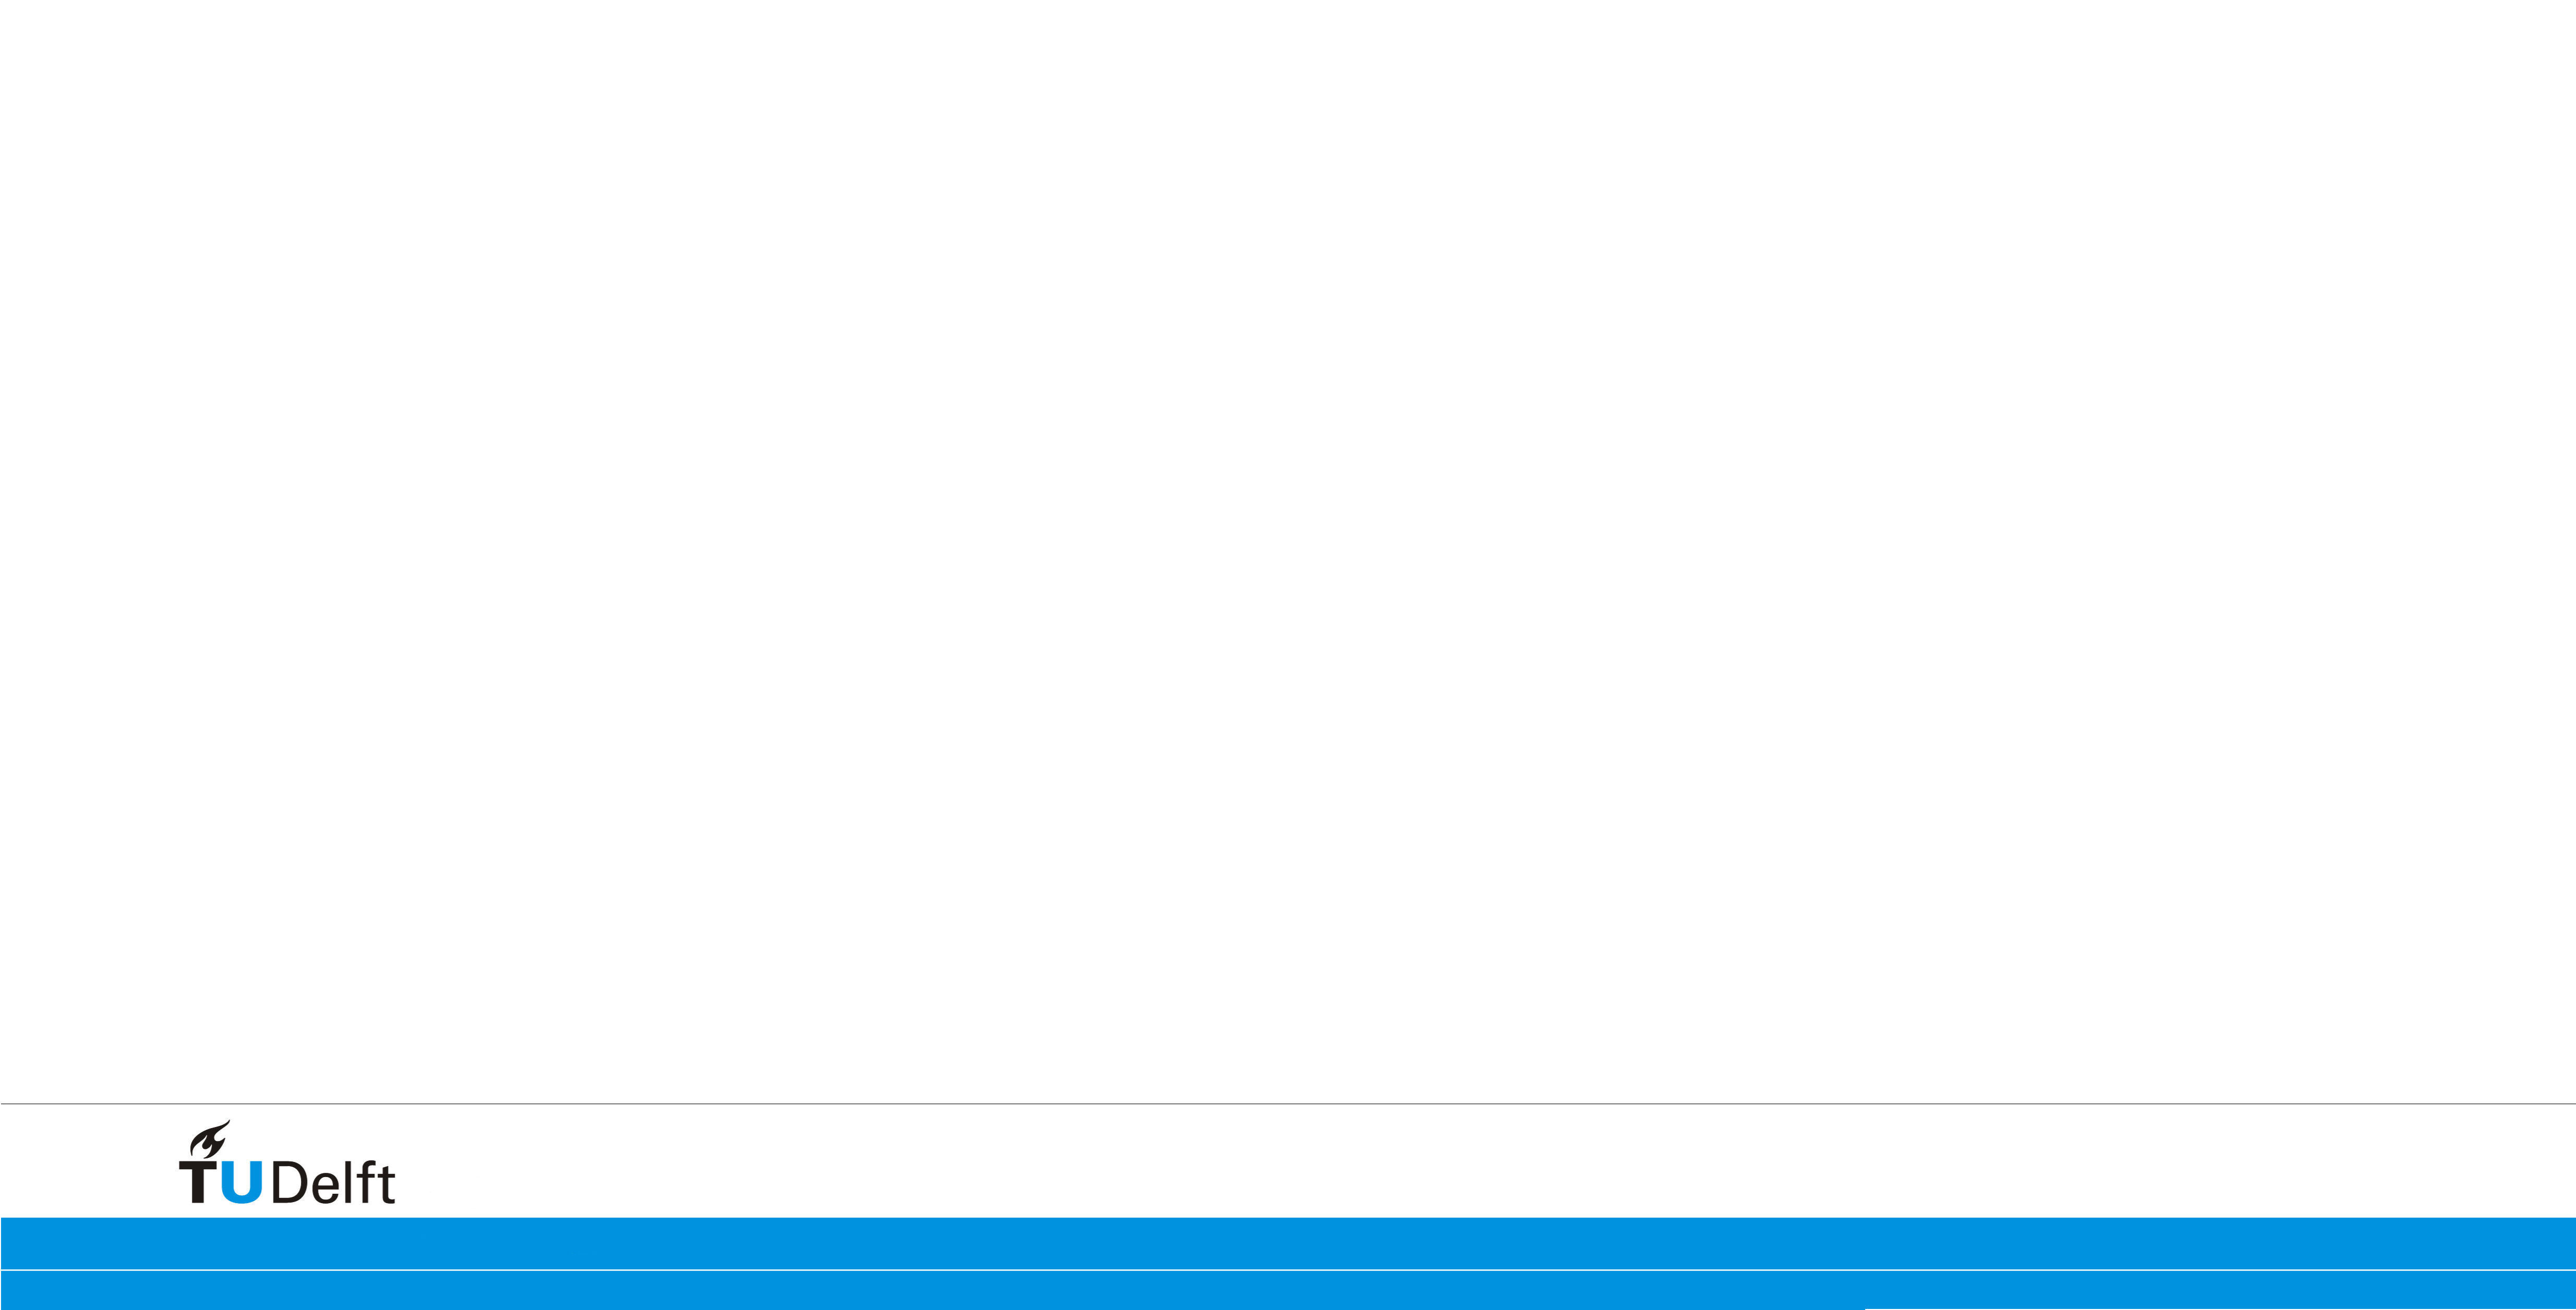
\includegraphics[scale=0.33]{TUDelft/beamer-tudelft-bies.jpg} }
\vskip-5pt}

\maketitle

\AtBeginSection[ ]
{
\begin{frame}{Outline}
    \tableofcontents[currentsection]
\end{frame}
}

\section{Motivation}
\begin{frame}{Motivation}
We want to map qubits on a quantum circuit (\textbf{virtual qubits}) to the qubits on a quantum chip (\textbf{physical qubits}).\\
\pause

\begin{figure}
     \centering
     \begin{subfigure}[b]{0.45\textwidth}
		\begin{overprint}
		\onslide<2-3>\centering
		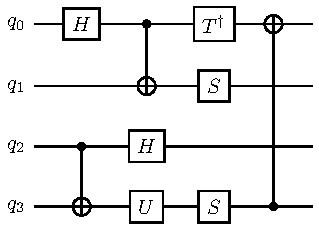
\includegraphics[height=60pt]{figures/default_circuit1}
		\onslide<4->\centering
		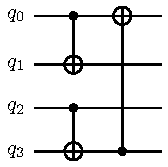
\includegraphics[height=60pt]{figures/default_circuit2}		
		\end{overprint}
     \end{subfigure}
     \hfill %\pause
     \begin{subfigure}[b]{0.45\textwidth}
		\begin{overprint}
		\onslide<3-4>\centering
		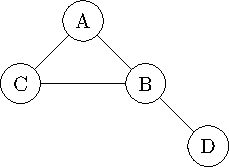
\includegraphics[scale=0.6]{figures/default_chip}
		\onslide<5>\centering
		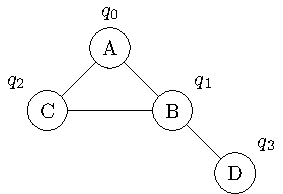
\includegraphics[scale=0.6]{figures/default_wrong}
		\onslide<6->\centering
		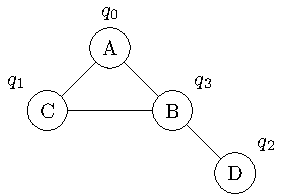
\includegraphics[scale=0.6]{figures/default_mapped}		
		\end{overprint}
     \end{subfigure}
     \hfill %\pause
\end{figure}
\pause


\end{frame}

\begin{frame}{Motivation}
Not always possible to find a mapping. Especially with a bigger circuit.\\
\pause
\begin{figure}
     \centering
     \begin{subfigure}[b]{0.45\textwidth}
		\begin{overprint}
		\onslide<2>\centering
		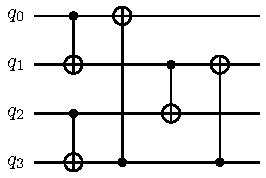
\includegraphics[height=60pt]{figures/extended_circuit}
		\onslide<3->\centering
		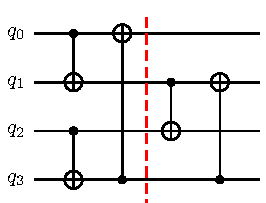
\includegraphics[height=60pt]{figures/default_circuit3}
		\end{overprint}
     \end{subfigure}
     \hfill %\pause
     \begin{subfigure}[b]{0.45\textwidth}
		\begin{overprint}
		\onslide<2-3>\centering
		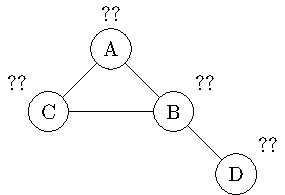
\includegraphics[scale=0.6]{figures/chip_unmapped}
		\onslide<4>\centering
		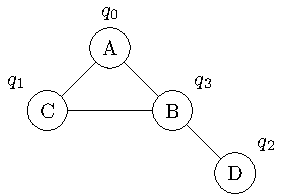
\includegraphics[scale=0.6]{figures/default_mapped}
		\onslide<5>\centering
		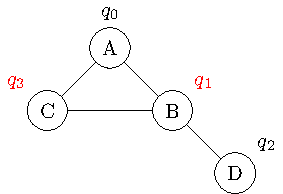
\includegraphics[scale=0.6]{figures/default_mapped2}
		\onslide<6->\centering
		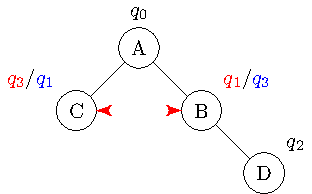
\includegraphics[scale=0.6]{figures/swapped_mapping}		
		\end{overprint}
     \end{subfigure}
     \hfill %\pause
\end{figure}
\pause
Map one part of the circuit. \pause \pause Map the next part of the circuit. \pause Move the qubits to go from one mapping to the next (Routing).

\end{frame}

\section{Methods}
\begin{frame}{Problem Setup}
	Given: A quantum circuit to map.
\pause
\begin{minipage}{0.5\textwidth}
\begin{figure}
     \centering
		\begin{overprint}
		\onslide<2>\centering
		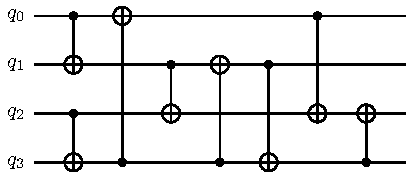
\includegraphics[width=0.9\textwidth]{figures/big_circuit}
		\onslide<3->\centering
		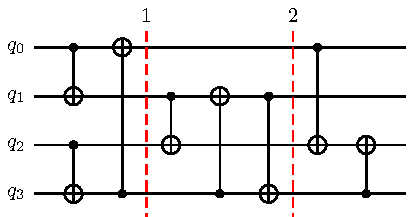
\includegraphics[width=0.9\textwidth]{figures/big_circuit_sliced}
		\end{overprint}
     \hfill %\pause
		\begin{overprint}
		\onslide<4>\centering
		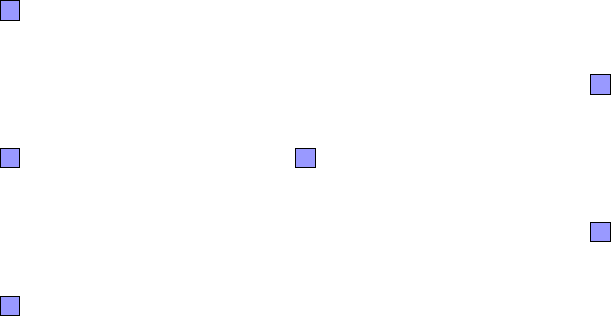
\includegraphics[width=0.7\textwidth]{figures/many_mappings}
		\onslide<5>\centering
		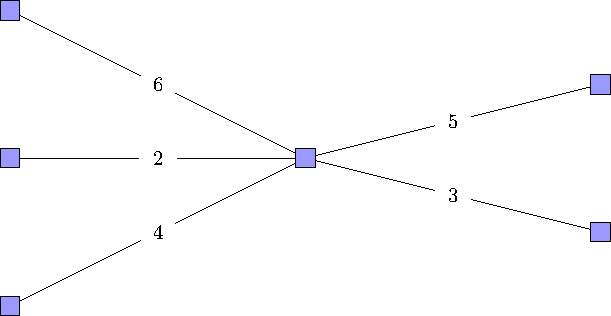
\includegraphics[width=0.7\textwidth]{figures/many_mappings_weights}
		\onslide<6->\centering
		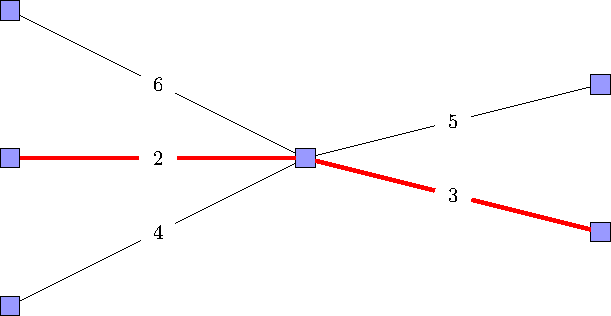
\includegraphics[width=0.7\textwidth]{figures/many_mappings_optimum}
		\end{overprint}
     \hfill %\pause
\end{figure}
\end{minipage}%
%
\begin{minipage}{0.5\textwidth}
\pause
Idea:
\begin{enumerate}
	\item Slice the circuit. \pause Get (multiple) mappings for each slice. \pause
	\item Estimate cost of changes. \pause
	\item Optimize the cost. \pause
\end{enumerate}
\end{minipage}%

Two part problem:\\
\begin{table}[]
\begin{tabular}{ll}
Initial Mapping: & Quantum Walk based search \pause \\
Routing:         & Classical Optimization   
\end{tabular}
\end{table}
\end{frame}

\begin{frame}{Solving Initial Mapping}\pause
It is a constraint satisfaction problem (CSP). \pause Classically, can do a backtracking search to find the solutions. \pause
\begin{figure}
     \centering
     \begin{subfigure}[b]{0.35\textwidth}
     \centering
     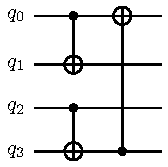
\includegraphics[scale=0.5]{figures/default_circuit2}
		\begin{overprint}
		\onslide<4>\centering
		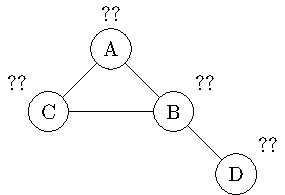
\includegraphics[width=0.7\textwidth]{figures/partial1}
		\onslide<5>\centering
		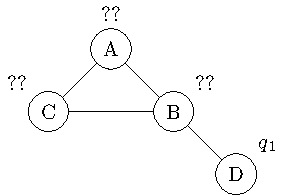
\includegraphics[width=0.7\textwidth]{figures/partial2}
		\onslide<6>\centering
		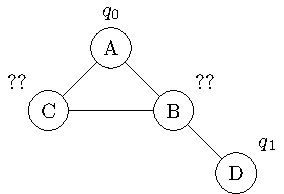
\includegraphics[width=0.7\textwidth]{figures/partial3}
		\onslide<7>\centering
		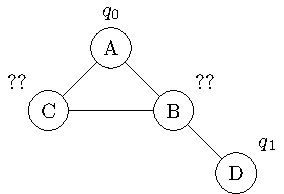
\includegraphics[width=0.7\textwidth]{figures/partial4}
		\onslide<8>\centering
		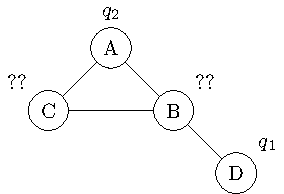
\includegraphics[width=0.7\textwidth]{figures/partial5}
		\onslide<9>\centering
		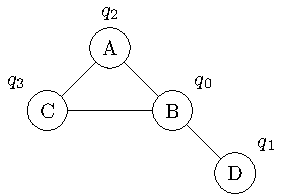
\includegraphics[width=0.7\textwidth]{figures/partial6}
		\onslide<10>\centering
		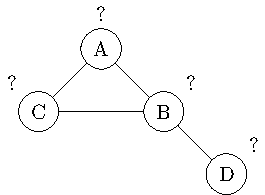
\includegraphics[width=0.7\textwidth]{figures/partial7}
		\end{overprint}
     \end{subfigure}
     \hfill %\pause
     \begin{subfigure}[b]{0.6\textwidth}
		\begin{overprint}
		\onslide<4>\centering
		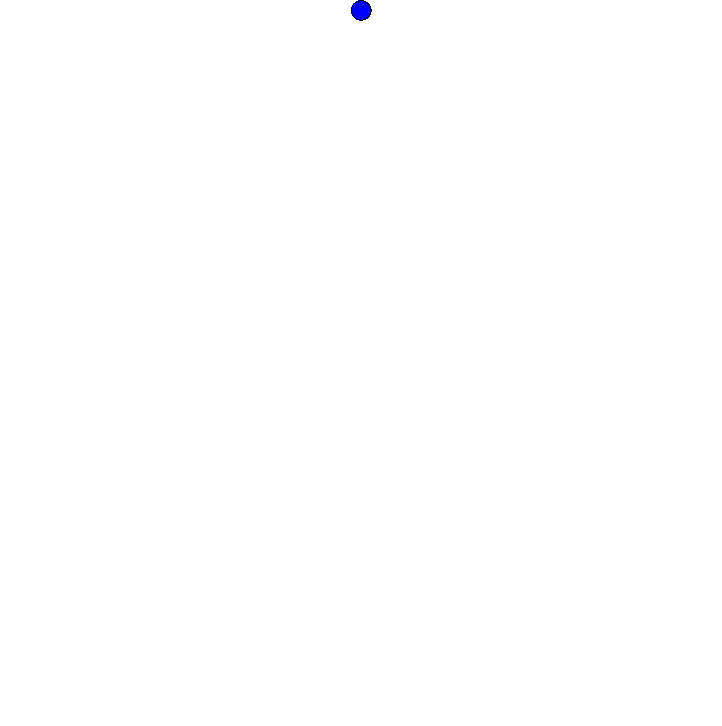
\includegraphics[height=120pt]{figures/tree1}
		\onslide<5>\centering
		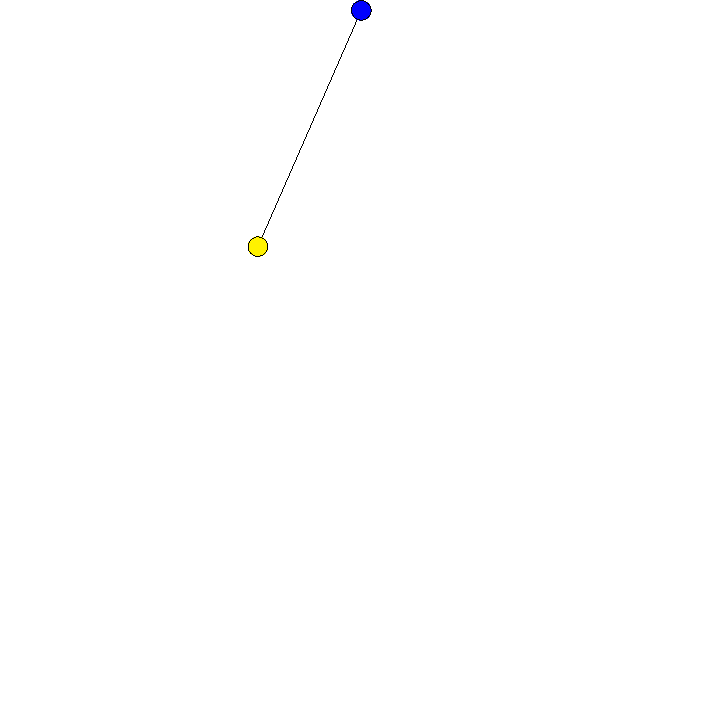
\includegraphics[height=120pt]{figures/tree2}
		\onslide<6>\centering
		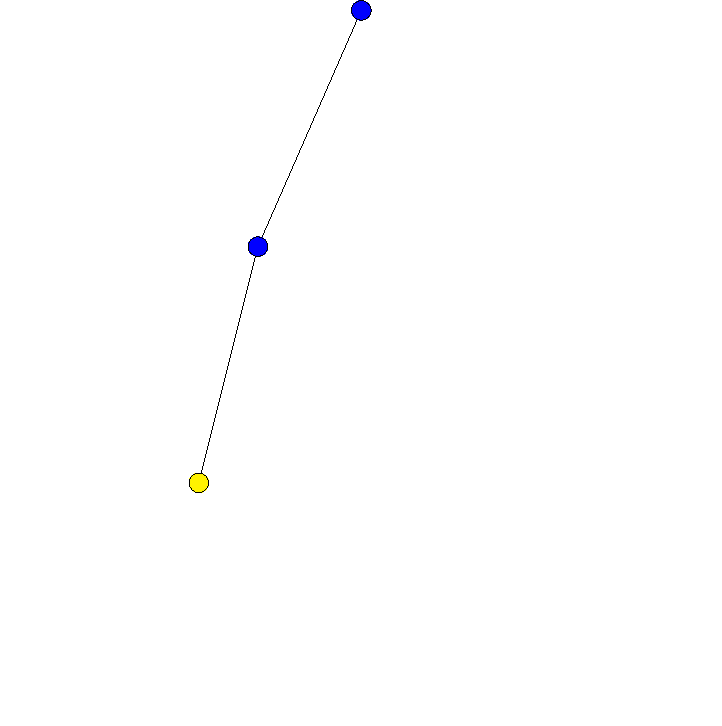
\includegraphics[height=120pt]{figures/tree3}
		\onslide<7>\centering
		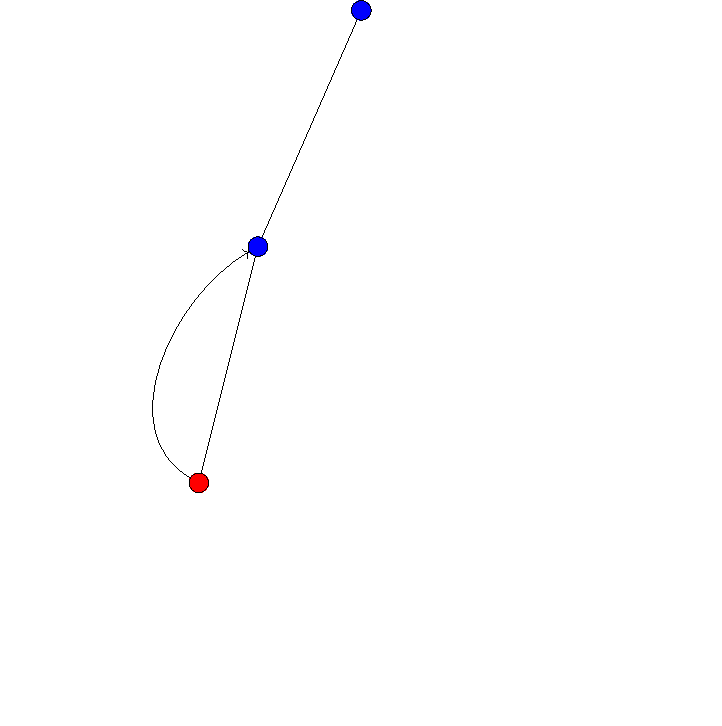
\includegraphics[height=120pt]{figures/tree4}
		\onslide<8>\centering
		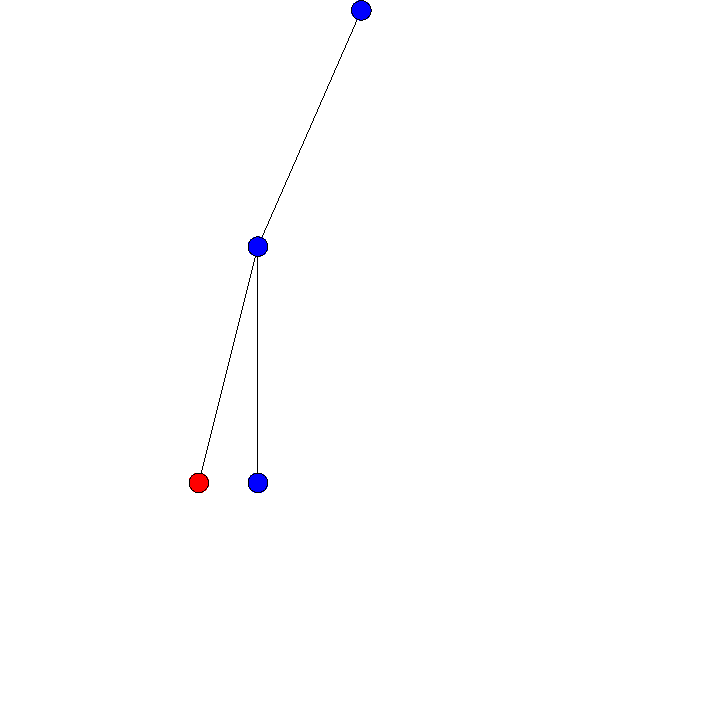
\includegraphics[height=120pt]{figures/tree5}
		\onslide<9>\centering
		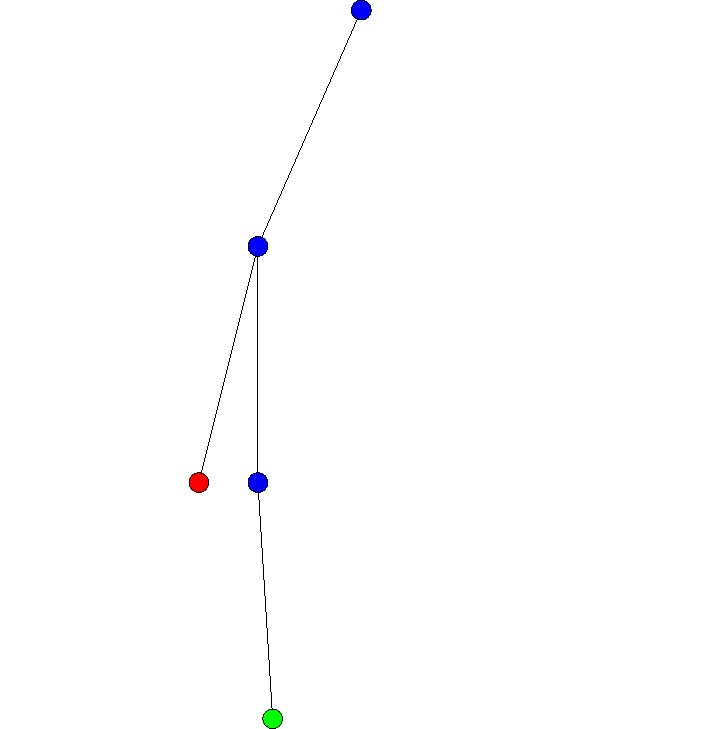
\includegraphics[height=120pt]{figures/tree6}
		\onslide<10->\centering
		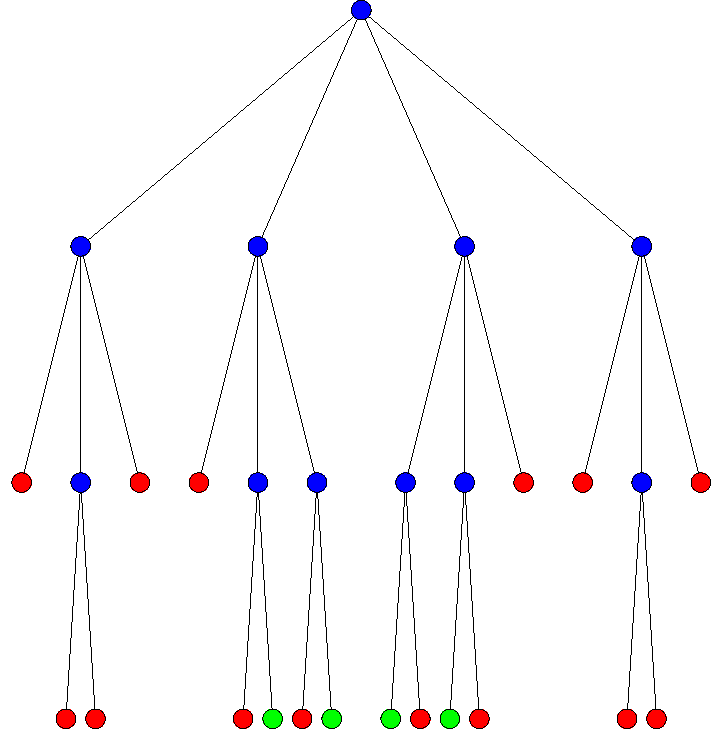
\includegraphics[height=120pt]{figures/tree7}	
		\end{overprint}
     \end{subfigure}
     \hfill %\pause
\end{figure}
\pause \pause \pause
Backtrack!!
\end{frame}

\begin{frame}{Quantum walk speed up}
	Speed up this backtracking for the CSP. \pause
	\begin{block}{Finding a solution \hfill {\small \texttt{(Montanaro, 2015)}}}
	Assume access to predicate $P(x) \rightarrow \text{\{true, false, indeterminate\}}$ \pause
	And heuristic $h$ to decide how to extend an assignment. \pause  \\
	
	A bounded error quantum algorithm evaluates $P$ and $h$ $\mathcal{O}(\sqrt{Tn^{\frac{5}{2}}}log(n))$ times each and outputs solution. \pause \\
	\end{block}
\begin{itemize}
	\item The backtracking tree is given implicitly using the predicate and heuristic.\pause
	\item In the worst case, $T$ grows as $n!$. We get a near quadratic separation between classical and quantum case.\pause
	\item Strike out previously found solutions to find \textcolor{red}{all} solutions.
\end{itemize}
	
\end{frame}

\begin{frame}{Quantum walk in a tree} \pause
The quantum walk operates on a $T$-dimensional Hilbert space spanned by $\{\ket{r} \cup \ket{x} x \in \{1, ..., T-1\}\}$ where $r$ is root. \pause \\
Walk starts in state $\ket{r}$ and is based on \textcolor{red}{diffusion operators} $D_x$. \pause
\begin{itemize}
		\item If $x$ is valid solution, then $D_x$ is identity.
	\pause
		\item If $x$ is indeterminate, and $ x \neq r $ then $D_x = \mathbb{I} - 2\ket{\psi_x}\bra{\psi_x} $ \\
		$$ \ket{\psi_x} \propto\left( \ket{x} + \sum_{y, x \to y} \ket{y} \right) $$
	\pause
		\item For the root, $ D_r = \mathbb{I} - 2\ket{\psi_r}\bra{\psi_r} $
		$$ \ket{\psi_r} \propto\left( \ket{r} + \sqrt{n}\sum_{y, r \to y} \ket{y} \right) $$
\end{itemize}

\end{frame}

\begin{frame}{Quantum walk in a tree}\pause
Let \textcolor{blue}{A} and \textcolor{red}{B} be the set of vertices even and odd distance from root, respectively.\pause

A step of the walk is applying \textcolor{red}{$R_B$}\textcolor{blue}{$R_A$} where \textcolor{blue}{$R_A$} = $\oplus_{x\in A}D_x$ and \textcolor{red}{$R_B$} = $\ket{r}\bra{r} + \oplus_{x\in B}D_x$\pause
\begin{figure}
	\centering
	\begin{overprint}
		\onslide<4>\centering
		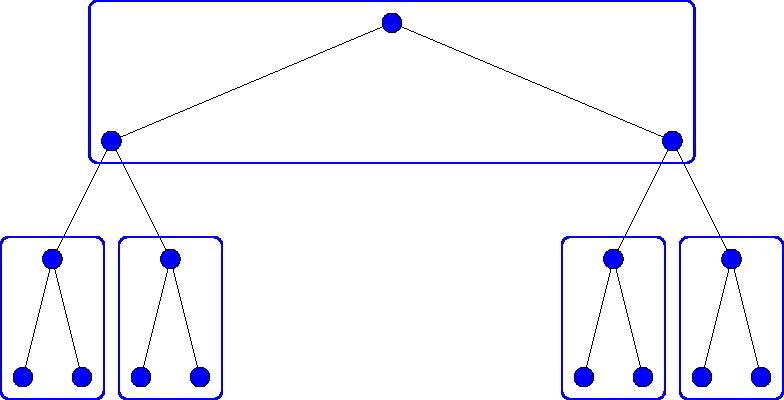
\includegraphics[height=120pt]{figures/R_A}
		\onslide<5>\centering
		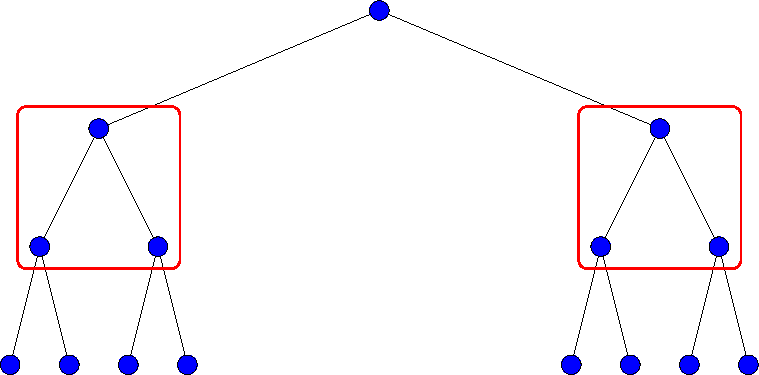
\includegraphics[height=120pt]{figures/R_B}
	\end{overprint}
\end{figure}
\end{frame}

\begin{frame}{Quantum Algorithm to detect solution}\pause
	\begin{block}{The algorithm \hfill {\small \texttt{(Montanaro, 2015)}}}
		Apply phase estimation to \textcolor{red}{$R_B$}\textcolor{blue}{$R_A$} on state $\ket{r}$ with precision $\mathcal{O}\left( \frac{1}{\sqrt{Tn}} \right)$. \pause \\
		If there is a solution, \textcolor{red}{$R_B$}\textcolor{blue}{$R_A$} has an eigenvector with eigenvalue 1 and overlap $\geq \frac{1}{2}$ with $\ket{r}$. \pause \\
		If there is no solution, $\lvert\lvert P_{\chi}\ket{r} \rvert\rvert^2 \leq \frac{1}{4}$ where $P_{\chi}$ is the projector onto the subspace spanned by eigenvectors of \textcolor{red}{$R_B$}\textcolor{blue}{$R_A$} with eigenvalue $e^{2i\theta}$ for $\theta \leq \frac{1}{2\sqrt{Tn}}$
	\end{block} \pause

Use the subroutine $K$ times and if the measured eigenvalue is 1 at least $\frac{3K}{8}$ times, a solution exists.
\end{frame}

\begin{frame}{Detection to search} \pause
\begin{itemize}
	\item Can use this detection procedure as a subroutine to \textcolor{blue}{find} the solutions in the tree via binary search. \pause
	\item Apply the procedure to the whole tree. \pause If it detects a solution, apply it to the subtree rooted at each of the children, and repeat. \pause 
\end{itemize}
\begin{figure}
	\centering
	\begin{overprint}
		\onslide<5>\centering
		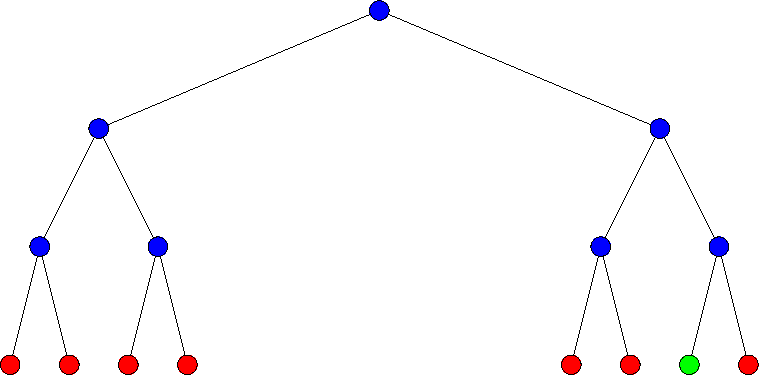
\includegraphics[height=100pt]{figures/search_tree1}
		\onslide<6>\centering
		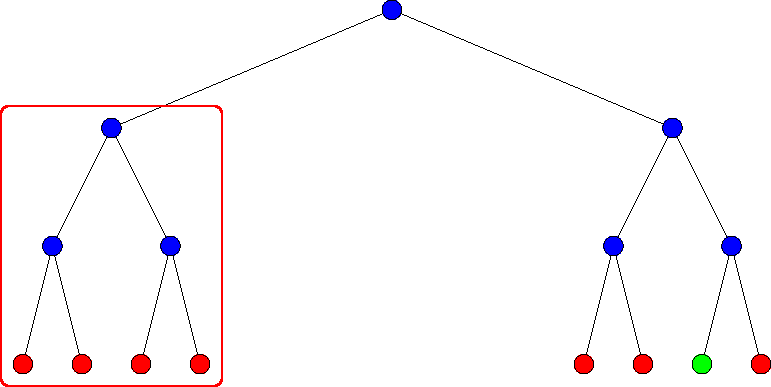
\includegraphics[height=100pt]{figures/search_tree2}
		\onslide<7->\centering
		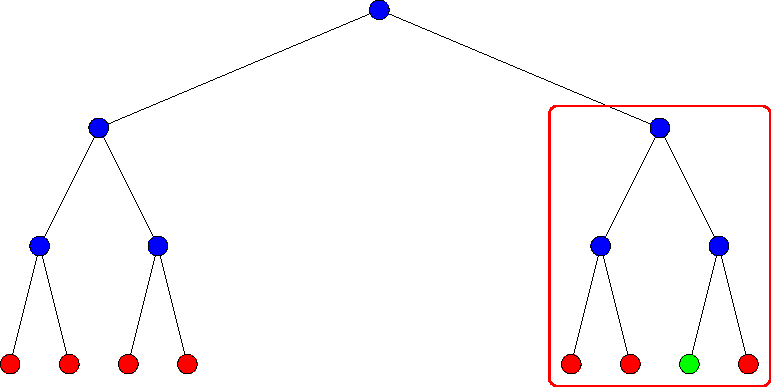
\includegraphics[height=100pt]{figures/search_tree3}
	\end{overprint}
\end{figure}
\end{frame}

\begin{frame}{Optimizations}
We propose a practical implementation of the method and further optimize both space and depth.\pause

\begin{block}{Depth optimization}\pause
	Eliminate dynamic heuristic $h$ and fix the order of qubit assignment. \pause \\
	Heuristic determines the shape of the tree.\pause \\
	Potentially a more efficient implementation of predicate by checking fewer constraints.
\end{block}\pause

\begin{alertblock}{More efficient encoding}\pause
	We propose a more efficient encoding of the partial assignment \pause \\
	$x_1 = v_1,...,x_l = v_l \rightarrow \ket{l}\ket{v_1}...\ket{v_l}\ket{*}...\ket{*}$ \pause \\
	Saves $nlog(n)$ qubits.
\end{alertblock}
\end{frame}

\begin{frame}{Slicing the circuit}
What if the detection algorithm returns "no solution exists"? \pause
\begin{figure}
	\centering
	\begin{overprint}
	\onslide<2>\centering
		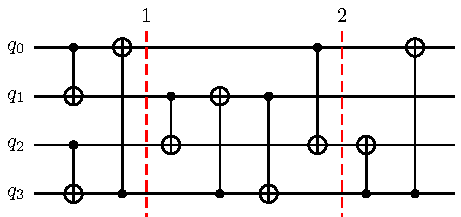
\includegraphics[height=80pt]{figures/wrong_sliced}
	\onslide<3->\centering
	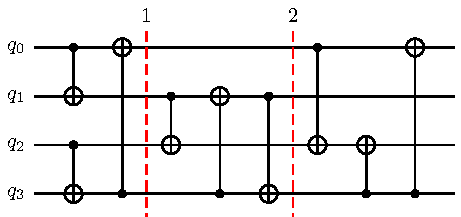
\includegraphics[height=80pt]{figures/right_sliced}
	\end{overprint}
\end{figure} \pause
Need to make the "slice" smaller.\pause \\
Proposed guess for size of slice = $d_{\text{G}}\cdot \lvert G_2 \rvert$\\
$d_{G} = \frac{\text{no. of edges}}{\text{no. of possible edges}}$, $\lvert G_2 \rvert = \text{no. of 2 qubit gates}$

\end{frame}

\begin{frame}{Optimizing Routing}\pause
What is the metric to be optimized? \pause \\
Distance measure between two mappings $\pi_1$ and $\pi_2$:
 $$ d_{\text{map}}(\pi_1, \pi_2) =  \sum_{\alpha \in Z} d_{\text{chip}}(\pi_1^{-1}(\alpha), \pi_2^{-1}(\alpha)) $$ \pause
\begin{figure}
     \centering
     \vspace{-0.2cm}
     \begin{subfigure}[b]{0.45\textwidth}
		\begin{overprint}
		\onslide<4-5>\centering
		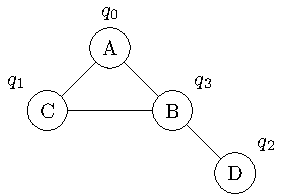
\includegraphics[scale=0.6]{figures/pi_1_1}
		\onslide<6>\centering
		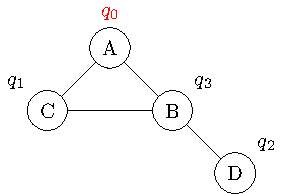
\includegraphics[scale=0.6]{figures/pi_1_2}
		\onslide<7>\centering
		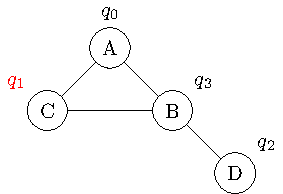
\includegraphics[scale=0.6]{figures/pi_1_3}
		\onslide<8>\centering
		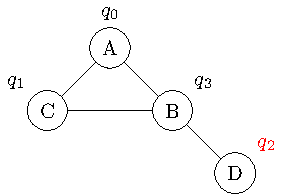
\includegraphics[scale=0.6]{figures/pi_1_4}
		\onslide<9>\centering
		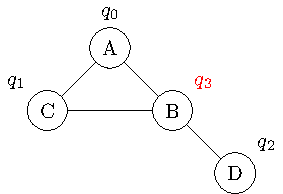
\includegraphics[scale=0.6]{figures/pi_1_5}
		\onslide<10->\centering
		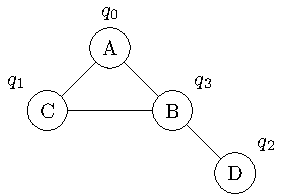
\includegraphics[scale=0.6]{figures/pi_1_6}
		\end{overprint}
     \end{subfigure}
     \hfill %\pause
     \begin{subfigure}[b]{0.45\textwidth}
		\begin{overprint}
		\onslide<4-5>\centering
		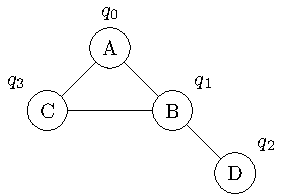
\includegraphics[scale=0.6]{figures/pi_2_1}	
		\onslide<6>\centering
		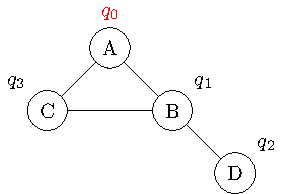
\includegraphics[scale=0.6]{figures/pi_2_2}
		\onslide<7>\centering
		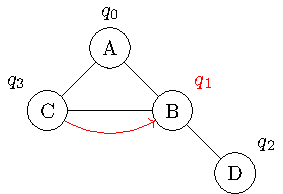
\includegraphics[scale=0.6]{figures/pi_2_3}
		\onslide<8>\centering
		\includegraphics[scale=0.6]{figures/pi_2_4}	
		\onslide<9>\centering
		\includegraphics[scale=0.6]{figures/pi_2_5}
		\onslide<10->\centering
		\includegraphics[scale=0.6]{figures/pi_2_6}		
		\end{overprint}
     \end{subfigure}
     \hfill %\pause
\end{figure}
\vspace{-1cm}
\begin{overprint}
	\onslide<5>\centering
	\begin{align*}
		d_{\text{map}}(\pi_1, \pi_2) =& d_{\text{c}}(\pi^{-1}_1(q_0),\pi^{-1}_2(q_0)) &+ d_{\text{c}}(\pi^{-1}_1(q_1),\pi^{-1}_2(q_1))\\
		+& d_{\text{c}}(\pi^{-1}_1(q_2),\pi^{-1}_2(q_2)) &+ d_{\text{c}}(\pi^{-1}_1(q_3),\pi^{-1}_2(q_3))
	\end{align*}
	\onslide<6>\centering
	\begin{align*}
		d_{\text{map}}(\pi_1, \pi_2) =& \text{\phantom{XXXXX}}0 &+ d_{\text{c}}(\pi^{-1}_1(q_1), \pi^{-1}_2(q_1))\\
		+& d_{\text{c}}(\pi^{-1}_1(q_2),\pi^{-1}_2(q_2)) &+ d_{\text{c}}(\pi^{-1}_1(q_3), \pi^{-1}_2(q_3))
	\end{align*}
	\onslide<7>\centering
	\begin{align*}
		d_{\text{map}}(\pi_1, \pi_2) =& \text{\phantom{XXXXX}}0 &+ \text{\phantom{XXXXX}}1\text{\phantom{XXXXXXXX}}&\\
		+& d_{\text{c}}(\pi^{-1}_1(q_2),\pi^{-1}_2(q_2)) &+ d_{\text{c}}(\pi^{-1}_1(q_3),\pi^{-1}_2(q_3))&
	\end{align*}
	\onslide<8>\centering
	\begin{align*}
		d_{\text{map}}(\pi_1, \pi_2) =& \text{\phantom{XXXXX}}0 &+ \text{\phantom{XXXXX}}1\text{\phantom{XXXXXXXX}}&\\
		+& \text{\phantom{XXXXX}}0 &+ d_{\text{c}}(\pi^{-1}_1(q_3),\pi^{-1}_2(q_3))&
	\end{align*}
	\onslide<9>\centering
	\begin{align*}
		d_{\text{map}}(\pi_1, \pi_2) =& \text{\phantom{XXXXX}}0 &+ \text{\phantom{XXXXX}}1\text{\phantom{XXXXXXXX}}&\\
		+& \text{\phantom{XXXXX}}0 &+ \text{\phantom{XXXXX}}1\text{\phantom{XXXXXXXX}}&
	\end{align*}
	\onslide<10->\centering
	\begin{align*}
		d_{\text{map}}(\pi_1, \pi_2) =& 2
	\end{align*}
\end{overprint}
\end{frame}

\begin{frame}{Optimizing Routing}
How to get the optimum "route"? \pause \\
Employ a simple greedy approach! \pause
\begin{figure}
	\begin{overprint}
		\onslide<3>\centering
		\includegraphics[scale=0.6]{figures/greedy1}
		\onslide<4>\centering
		\includegraphics[scale=0.6]{figures/greedy2}
		\onslide<5->\centering
		\includegraphics[scale=0.6]{figures/greedy3}
	\end{overprint}
\end{figure}
\pause \pause \pause
Potentially miss global optimum but we avoid combinatorial explosion.
\end{frame}

\section{Results}
\begin{frame}{Results}\pause
\begin{itemize}
	\item Effect of choice of heuristic $h$:\\
	\begin{figure}
	\centering
		\includegraphics[scale=0.6]{figures/heuristic} 
	\end{figure}
\end{itemize}
\end{frame}

\begin{frame}{Results}
\begin{block}{Benchmarking}\pause
Performance benchmarked against classical mappers for actual circuits (RevLib\footnote{Wille, 2008}) \pause \\
Analysed the number of SWAPs needed.\\
Best performance matches QMAP\footnote{Lao et. al., 2022} for small circuits (~5 qubits, ~30 CNOTs). \pause \\
Performance detoriates for bigger circuits, upto \textcolor{red}{80\%} more SWAPs needed.
\end{block}
\end{frame}

\begin{frame}{Results}
	\begin{figure}
	\centering
	\begin{subfigure}{0.48\textwidth}
	\centering
		\includegraphics[width=\textwidth]{figures/R_vs_d}
	\end{subfigure}
	\begin{subfigure}{0.48\textwidth}
	\centering
		\includegraphics[width=\textwidth]{figures/R_vs_n}
	\end{subfigure}
	\end{figure}
\end{frame}

\section{Conclusions}
\begin{frame}{Conclusions}\pause
\begin{itemize}
	\item Proposed a new model for qubit mapping based on CSP and combinatorial optimization. \pause
	\item Provided a practical implementation of a quantum algorithm for (initial) qubit mapping. \pause
	\item Further, optimized both the space and depth by eliminating dynamic heuristic and using a more efficient encoding. \pause
	\item Benchmarked and compared the depth overhead to other classical mapping and routing algorithms.
\end{itemize}

\end{frame}

\begin{frame}
 \begin{center}
  Thanks!
 \end{center}

\end{frame}

\end{document}
